% ═══════════════════════════════════════════════════════════════════════════════
% OpenMagnetics Professional Power Inductor Datasheet
% ═══════════════════════════════════════════════════════════════════════════════
% Industry-standard format inspired by Coilcraft, Würth Elektronik, TDK
% Compatible with LatexReportGenerator template tag replacement
%
% Version: 2.0
% ═══════════════════════════════════════════════════════════════════════════════

\documentclass[10pt,a4paper]{article}

% ═══════════════════════════════════════════════════════════════════════════════
% PACKAGES
% ═══════════════════════════════════════════════════════════════════════════════
\usepackage[utf8]{inputenc}
\usepackage[T1]{fontenc}
\usepackage{helvet}                   % Professional sans-serif font
\renewcommand{\familydefault}{\sfdefault}
\usepackage{geometry}
\usepackage{graphicx}
\usepackage{booktabs}
\usepackage{xcolor}
\usepackage{array}
\usepackage{fancyhdr}
\usepackage{tikz}
\usepackage{colortbl}
\usepackage{multirow}
\usepackage{tabularx}
\usepackage{float}
\usepackage{siunitx}                  % SI units formatting
\usepackage{hyperref}
\usepackage{enumitem}
\usepackage{tcolorbox}
\usepackage{calc}

\usetikzlibrary{shapes,arrows,positioning,calc}

% ═══════════════════════════════════════════════════════════════════════════════
% DOCUMENT SETUP
% ═══════════════════════════════════════════════════════════════════════════════
\geometry{left=12mm, right=12mm, top=15mm, bottom=15mm}
\setlength{\parindent}{0pt}
\setlength{\parskip}{0pt}

% Color definitions (professional blue/gray scheme)
\definecolor{primary}{RGB}{0, 63, 135}        % Deep professional blue
\definecolor{secondary}{RGB}{0, 102, 178}     % Lighter blue for accents
\definecolor{accent}{RGB}{0, 150, 136}        % Teal for highlights
\definecolor{lightbg}{RGB}{245, 248, 250}     % Light gray-blue background
\definecolor{gridbg}{RGB}{235, 240, 245}      % Alternating row color
\definecolor{textdark}{RGB}{33, 37, 41}       % Dark text
\definecolor{textmuted}{RGB}{108, 117, 125}   % Muted text
\definecolor{success}{RGB}{40, 167, 69}       % Green for compliance
\definecolor{warning}{RGB}{255, 193, 7}       % Yellow for notes

% ═══════════════════════════════════════════════════════════════════════════════
% HEADER AND FOOTER
% ═══════════════════════════════════════════════════════════════════════════════
\pagestyle{fancy}
\fancyhf{}
\fancyhead[L]{\footnotesize\color{textmuted}{{COMPANY_NAME}}}
\fancyhead[C]{\footnotesize\textbf{\color{primary}{{PART_NUMBER}}} - Power Inductor}
\fancyhead[R]{\footnotesize\color{textmuted}Rev. {{REVISION}}}
\fancyfoot[L]{\footnotesize\color{textmuted}Generated by OpenMagnetics}
\fancyfoot[C]{\footnotesize\color{textmuted}\thepage\ of \pageref{LastPage}}
\fancyfoot[R]{\footnotesize\color{textmuted}\today}
\renewcommand{\headrulewidth}{0.4pt}
\renewcommand{\footrulewidth}{0.4pt}

% ═══════════════════════════════════════════════════════════════════════════════
% CUSTOM COMMANDS
% ═══════════════════════════════════════════════════════════════════════════════
\newcommand{\sectiontitle}[1]{%
    \vspace{3mm}%
    {\large\bfseries\color{primary}#1}%
    \vspace{1mm}%
    \hrule height 0.3pt%
    \vspace{2mm}%
}

\newcommand{\specvalue}[1]{\textbf{#1}}

\newcolumntype{L}[1]{>{\raggedright\arraybackslash}p{#1}}
\newcolumntype{C}[1]{>{\centering\arraybackslash}p{#1}}
\newcolumntype{R}[1]{>{\raggedleft\arraybackslash}p{#1}}

% ═══════════════════════════════════════════════════════════════════════════════
% DOCUMENT START
% ═══════════════════════════════════════════════════════════════════════════════
\begin{document}

% ═══════════════════════════════════════════════════════════════════════════════
% HEADER BANNER
% ═══════════════════════════════════════════════════════════════════════════════
\begin{tikzpicture}[remember picture, overlay]
    \fill[primary] (current page.north west) rectangle ([yshift=-25mm]current page.north east);
\end{tikzpicture}

\vspace*{-8mm}
\begin{minipage}[t]{0.65\textwidth}
    \color{white}
    {\fontsize{24}{28}\selectfont\bfseries {{PART_NUMBER}}}\\[3mm]
    {\large {{PART_DESCRIPTION}}}\\[1mm]
    {\normalsize Power Inductor / Filter Choke}
\end{minipage}
\hfill
\begin{minipage}[t]{0.30\textwidth}
    \raggedleft
    \color{white}
    {\large\bfseries {{COMPANY_NAME}}}\\[2mm]
    % Logo placeholder - replace with actual logo
    % \includegraphics[width=30mm]{logo.png}
\end{minipage}

\vspace{10mm}

% ═══════════════════════════════════════════════════════════════════════════════
% KEY PARAMETERS HIGHLIGHT BOX
% ═══════════════════════════════════════════════════════════════════════════════
\begin{tcolorbox}[
    colback=lightbg,
    colframe=primary,
    boxrule=0.5pt,
    arc=2mm,
    left=4mm,
    right=4mm,
    top=3mm,
    bottom=3mm
]
\centering
\renewcommand{\arraystretch}{1.4}
\begin{tabular}{C{30mm}C{30mm}C{30mm}C{30mm}C{30mm}}
    \textcolor{textmuted}{\footnotesize Inductance} & 
    \textcolor{textmuted}{\footnotesize DC Resistance} & 
    \textcolor{textmuted}{\footnotesize Saturation Current} & 
    \textcolor{textmuted}{\footnotesize RMS Current} & 
    \textcolor{textmuted}{\footnotesize Core Shape} \\
    {\Large\bfseries\color{primary} {{MAGNETIZING_INDUCTANCE_UH}}} & 
    {\Large\bfseries\color{primary} TBD} & 
    {\Large\bfseries\color{primary} TBD} & 
    {\Large\bfseries\color{primary} TBD} & 
    {\Large\bfseries\color{primary} {{CORE_SHAPE}}} \\
    \textcolor{textmuted}{\footnotesize $\mu$H $\pm$20\%} & 
    \textcolor{textmuted}{\footnotesize m$\Omega$ max} & 
    \textcolor{textmuted}{\footnotesize A (30\% drop)} & 
    \textcolor{textmuted}{\footnotesize A ($\Delta T$=40°C)} & 
    \textcolor{textmuted}{\footnotesize} \\
\end{tabular}
\end{tcolorbox}

\vspace{3mm}

% ═══════════════════════════════════════════════════════════════════════════════
% TWO-COLUMN LAYOUT: FEATURES/APPLICATIONS + IMAGE
% ═══════════════════════════════════════════════════════════════════════════════
\begin{minipage}[t]{0.48\textwidth}
    \sectiontitle{Features}
    \begin{itemize}[leftmargin=4mm, itemsep=1pt, topsep=0pt]
        \item High saturation current capability
        \item Low DC resistance for efficiency
        \item Excellent thermal performance
        \item Soft saturation characteristic (if ferrite/powder)
        \item Magnetically shielded construction
        \item AEC-Q200 qualified (automotive grade)
    \end{itemize}
    
    \vspace{2mm}
    \sectiontitle{Applications}
    \begin{itemize}[leftmargin=4mm, itemsep=1pt, topsep=0pt]
        \item DC-DC Buck/Boost Converters
        \item Power Factor Correction (PFC)
        \item Point-of-Load (POL) Regulators
        \item Solar/Wind Power Inverters
        \item EV/HEV Power Electronics
        \item Industrial Motor Drives
    \end{itemize}
\end{minipage}
\hfill
\begin{minipage}[t]{0.48\textwidth}
    \centering
    % Component image placeholder
    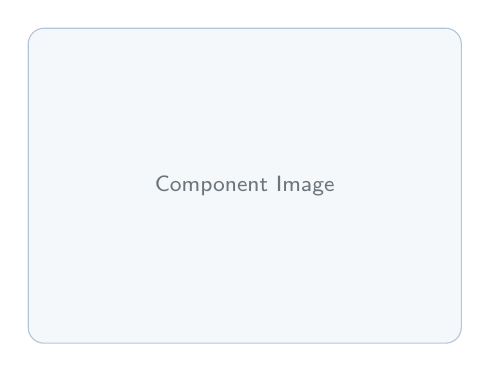
\begin{tikzpicture}
        \draw[rounded corners=2mm, fill=lightbg, draw=primary!30] (0,0) rectangle (55mm, 40mm);
        \node[text=textmuted] at (27.5mm, 20mm) {\footnotesize Component Image};
        % Replace with: \includegraphics[width=55mm]{component_image.png}
    \end{tikzpicture}
    
    \vspace{2mm}
    {\footnotesize\color{textmuted} {{CORE_SHAPE}} - {{CORE_MATERIAL}}}
\end{minipage}

\vspace{4mm}

% ═══════════════════════════════════════════════════════════════════════════════
% ELECTRICAL SPECIFICATIONS
% ═══════════════════════════════════════════════════════════════════════════════
\sectiontitle{Electrical Specifications}

\renewcommand{\arraystretch}{1.25}
{\footnotesize
\begin{tabular}{|L{45mm}|C{12mm}|C{22mm}|C{22mm}|C{22mm}|C{15mm}|L{32mm}|}
\hline
\rowcolor{primary}
\textcolor{white}{\textbf{Parameter}} & 
\textcolor{white}{\textbf{Symbol}} & 
\textcolor{white}{\textbf{Min}} & 
\textcolor{white}{\textbf{Typ}} & 
\textcolor{white}{\textbf{Max}} & 
\textcolor{white}{\textbf{Unit}} & 
\textcolor{white}{\textbf{Conditions}} \\
\hline
Inductance & $L$ & - & \specvalue{{{MAGNETIZING_INDUCTANCE_UH}}} & - & $\mu$H & 0 A DC, 100 kHz \\
\rowcolor{gridbg}
Inductance Tolerance & - & -20 & - & +20 & \% & \\
DC Resistance & $R_{DC}$ & - & - & TBD & m$\Omega$ & 25°C \\
\rowcolor{gridbg}
Saturation Current & $I_{sat}$ & - & - & TBD & A & L drops 30\% \\
RMS Current & $I_{rms}$ & - & - & TBD & A & $\Delta T$ = 40°C \\
\rowcolor{gridbg}
Self-Resonant Frequency & SRF & TBD & - & - & MHz & \\
Operating Frequency & $f_{op}$ & - & {{OPERATING_FREQUENCY_KHZ}} & 1000 & kHz & \\
\hline
\end{tabular}
}

\vspace{4mm}

% ═══════════════════════════════════════════════════════════════════════════════
% TWO-COLUMN: CORE DATA + WINDING DATA
% ═══════════════════════════════════════════════════════════════════════════════
\begin{minipage}[t]{0.48\textwidth}
\sectiontitle{Core Data}
{\footnotesize
\begin{tabular}{|L{35mm}|L{25mm}|}
\hline
\rowcolor{primary}
\textcolor{white}{\textbf{Parameter}} & \textcolor{white}{\textbf{Value}} \\
\hline
Core Shape & {{CORE_SHAPE}} \\
\rowcolor{gridbg}
Core Material & {{CORE_MATERIAL}} \\
Effective Area ($A_e$) & {{EFFECTIVE_AREA_MM2}} mm² \\
\rowcolor{gridbg}
Effective Length ($l_e$) & {{EFFECTIVE_LENGTH_MM}} mm \\
Effective Volume ($V_e$) & {{EFFECTIVE_VOLUME_MM3}} mm³ \\
\rowcolor{gridbg}
Air Gap Length & {{GAP_LENGTH_MM}} mm \\
Number of Gaps & {{NUMBER_GAPS}} \\
\hline
\end{tabular}
}
\end{minipage}
\hfill
\begin{minipage}[t]{0.48\textwidth}
\sectiontitle{Winding Construction}
{\footnotesize
\begin{tabular}{|L{35mm}|L{25mm}|}
\hline
\rowcolor{primary}
\textcolor{white}{\textbf{Parameter}} & \textcolor{white}{\textbf{Value}} \\
\hline
Number of Turns & {{NUMBER_TURNS_W1}} \\
\rowcolor{gridbg}
Number of Parallels & {{NUMBER_PARALLELS_W1}} \\
Wire Type & {{WIRE_TYPE_W1}} \\
\rowcolor{gridbg}
Conductor Diameter & {{WIRE_DIAMETER_W1}} mm \\
Number of Layers & TBD \\
\rowcolor{gridbg}
Fill Factor & TBD \% \\
\hline
\end{tabular}
}
\end{minipage}

\vspace{4mm}

% ═══════════════════════════════════════════════════════════════════════════════
% PERFORMANCE ANALYSIS
% ═══════════════════════════════════════════════════════════════════════════════
\sectiontitle{Performance Analysis}

\begin{minipage}[t]{0.48\textwidth}
{\footnotesize
Test Conditions: $f$ = {{OPERATING_FREQUENCY_KHZ}} kHz, $T_{amb}$ = {{AMBIENT_TEMPERATURE}}

\vspace{2mm}
\begin{tabular}{|L{35mm}|L{25mm}|}
\hline
\rowcolor{primary}
\textcolor{white}{\textbf{Loss Component}} & \textcolor{white}{\textbf{Value}} \\
\hline
Core Losses ($P_{core}$) & {{CORE_LOSSES}} \\
\rowcolor{gridbg}
Winding Losses ($P_{cu}$) & {{WINDING_LOSSES}} \\
\textbf{Total Losses} & \textbf{{{TOTAL_LOSSES}}} \\
\hline
\rowcolor{gridbg}
Peak Flux Density ($B_{pk}$) & {{PEAK_FLUX_DENSITY_MT}} mT \\
Max Surface Temperature & {{MAX_TEMPERATURE}} °C \\
\hline
\end{tabular}
}
\end{minipage}
\hfill
\begin{minipage}[t]{0.48\textwidth}
\centering
% Winding cross-section placeholder
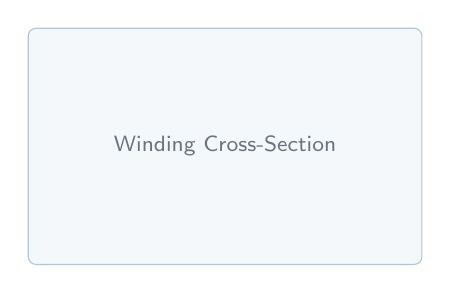
\begin{tikzpicture}
    \draw[rounded corners=1mm, fill=lightbg, draw=primary!30] (0,0) rectangle (50mm, 30mm);
    \node[text=textmuted] at (25mm, 15mm) {\footnotesize Winding Cross-Section};
\end{tikzpicture}
\end{minipage}

\vspace{4mm}

% ═══════════════════════════════════════════════════════════════════════════════
% CHARACTERISTIC CURVES
% ═══════════════════════════════════════════════════════════════════════════════
\sectiontitle{Characteristic Curves}

\begin{minipage}[t]{0.32\textwidth}
\centering
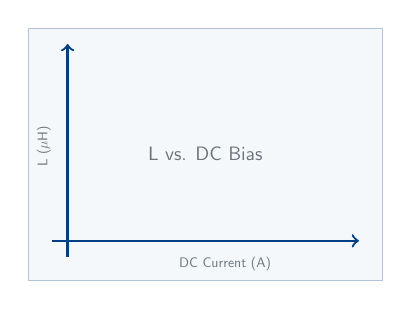
\begin{tikzpicture}
    \draw[fill=lightbg, draw=primary!30] (0,0) rectangle (45mm, 32mm);
    \draw[primary, thick, ->] (3mm, 5mm) -- (42mm, 5mm) node[right, scale=0.6] {};
    \draw[primary, thick, ->] (5mm, 3mm) -- (5mm, 30mm) node[above, scale=0.6] {};
    \node[text=textmuted, scale=0.7] at (22.5mm, 16mm) {L vs. DC Bias};
    \node[text=textmuted, scale=0.5] at (25mm, 2mm) {DC Current (A)};
    \node[text=textmuted, scale=0.5, rotate=90] at (2mm, 17mm) {L ($\mu$H)};
\end{tikzpicture}
\end{minipage}
\hfill
\begin{minipage}[t]{0.32\textwidth}
\centering
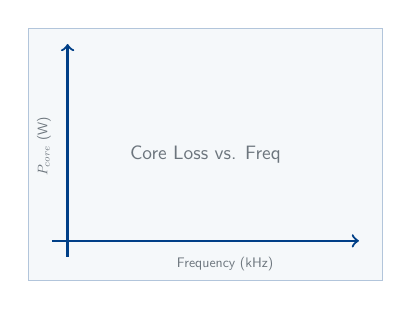
\begin{tikzpicture}
    \draw[fill=lightbg, draw=primary!30] (0,0) rectangle (45mm, 32mm);
    \draw[primary, thick, ->] (3mm, 5mm) -- (42mm, 5mm);
    \draw[primary, thick, ->] (5mm, 3mm) -- (5mm, 30mm);
    \node[text=textmuted, scale=0.7] at (22.5mm, 16mm) {Core Loss vs. Freq};
    \node[text=textmuted, scale=0.5] at (25mm, 2mm) {Frequency (kHz)};
    \node[text=textmuted, scale=0.5, rotate=90] at (2mm, 17mm) {$P_{core}$ (W)};
\end{tikzpicture}
\end{minipage}
\hfill
\begin{minipage}[t]{0.32\textwidth}
\centering
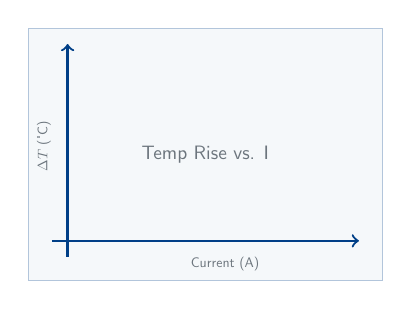
\begin{tikzpicture}
    \draw[fill=lightbg, draw=primary!30] (0,0) rectangle (45mm, 32mm);
    \draw[primary, thick, ->] (3mm, 5mm) -- (42mm, 5mm);
    \draw[primary, thick, ->] (5mm, 3mm) -- (5mm, 30mm);
    \node[text=textmuted, scale=0.7] at (22.5mm, 16mm) {Temp Rise vs. I};
    \node[text=textmuted, scale=0.5] at (25mm, 2mm) {Current (A)};
    \node[text=textmuted, scale=0.5, rotate=90] at (2mm, 17mm) {$\Delta T$ (°C)};
\end{tikzpicture}
\end{minipage}

\vspace{4mm}

% ═══════════════════════════════════════════════════════════════════════════════
% ENVIRONMENTAL & COMPLIANCE
% ═══════════════════════════════════════════════════════════════════════════════
\begin{minipage}[t]{0.48\textwidth}
\sectiontitle{Environmental Specifications}
{\footnotesize
\begin{tabular}{|L{35mm}|L{25mm}|}
\hline
\rowcolor{primary}
\textcolor{white}{\textbf{Parameter}} & \textcolor{white}{\textbf{Specification}} \\
\hline
Operating Temperature & -40 to +125°C \\
\rowcolor{gridbg}
Storage Temperature & -40 to +150°C \\
Humidity & 95\% RH max \\
\rowcolor{gridbg}
Vibration & 20g, 10-2000 Hz \\
MTBF & $>$1,000,000 hours \\
\hline
\end{tabular}
}
\end{minipage}
\hfill
\begin{minipage}[t]{0.48\textwidth}
\sectiontitle{Compliance \& Certifications}
\begin{itemize}[leftmargin=4mm, itemsep=0pt, topsep=0pt]
    \item[\textcolor{success}{\checkmark}] RoHS 2015/863/EU Compliant
    \item[\textcolor{success}{\checkmark}] REACH SVHC Compliant
    \item[\textcolor{success}{\checkmark}] Halogen-Free (IEC 61249-2-21)
    \item[\textcolor{success}{\checkmark}] AEC-Q200 Qualified (Automotive)
    \item[\textcolor{success}{\checkmark}] UL Recognized (E12345)
\end{itemize}
\end{minipage}

\vspace{4mm}

% ═══════════════════════════════════════════════════════════════════════════════
% DIMENSIONS & PACKAGING
% ═══════════════════════════════════════════════════════════════════════════════
\sectiontitle{Package Dimensions}

\begin{minipage}[t]{0.55\textwidth}
\centering
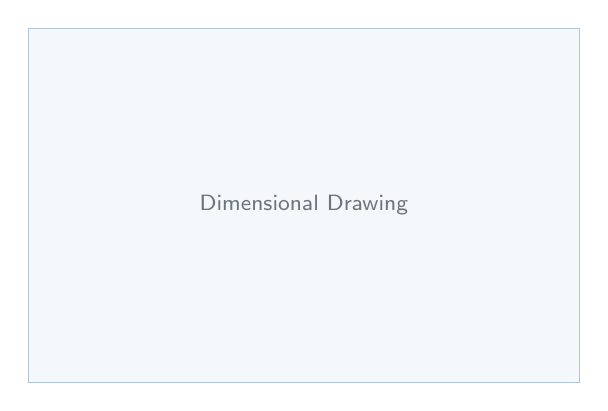
\begin{tikzpicture}
    \draw[fill=lightbg, draw=primary!30] (0,0) rectangle (70mm, 45mm);
    \node[text=textmuted] at (35mm, 22.5mm) {\footnotesize Dimensional Drawing};
    % Replace with actual drawing or: \includegraphics[width=70mm]{dimensions.png}
\end{tikzpicture}
\end{minipage}
\hfill
\begin{minipage}[t]{0.42\textwidth}
{\footnotesize
\begin{tabular}{|L{20mm}|C{15mm}|C{12mm}|}
\hline
\rowcolor{primary}
\textcolor{white}{\textbf{Dimension}} & \textcolor{white}{\textbf{Value}} & \textcolor{white}{\textbf{Tol.}} \\
\hline
Length (A) & TBD & $\pm$0.5 \\
\rowcolor{gridbg}
Width (B) & TBD & $\pm$0.5 \\
Height (C) & TBD & $\pm$0.5 \\
\rowcolor{gridbg}
Lead Spacing & TBD & $\pm$0.3 \\
Lead Diameter & TBD & $\pm$0.05 \\
\rowcolor{gridbg}
Weight & TBD g & - \\
\hline
\end{tabular}
}

\vspace{3mm}
{\footnotesize\color{textmuted} All dimensions in mm unless noted.}
\end{minipage}

\vspace{4mm}

% ═══════════════════════════════════════════════════════════════════════════════
% ORDERING INFORMATION
% ═══════════════════════════════════════════════════════════════════════════════
\sectiontitle{Ordering Information}

{\footnotesize
\begin{tabular}{|L{35mm}|C{25mm}|C{20mm}|C{25mm}|C{20mm}|C{20mm}|}
\hline
\rowcolor{primary}
\textcolor{white}{\textbf{Part Number}} & 
\textcolor{white}{\textbf{Inductance}} & 
\textcolor{white}{\textbf{Tolerance}} & 
\textcolor{white}{\textbf{Packaging}} & 
\textcolor{white}{\textbf{MOQ}} &
\textcolor{white}{\textbf{Lead Time}} \\
\hline
{{PART_NUMBER}} & {{MAGNETIZING_INDUCTANCE_UH}} $\mu$H & $\pm$20\% & Bulk / T\&R & 100 & Stock \\
\hline
\end{tabular}
}

\vspace{3mm}

% ═══════════════════════════════════════════════════════════════════════════════
% FOOTER NOTES
% ═══════════════════════════════════════════════════════════════════════════════
\begin{tcolorbox}[
    colback=warning!10,
    colframe=warning!50,
    boxrule=0.3pt,
    arc=1mm,
    left=3mm,
    right=3mm,
    top=2mm,
    bottom=2mm
]
{\footnotesize\color{textdark}
\textbf{Important Notice:} Specifications are subject to change without notice. Always verify current specifications before design-in. Refer to application notes for derating curves and design guidelines. For custom designs, contact {{COMPANY_NAME}} engineering support.
}
\end{tcolorbox}

\vspace{2mm}
{\footnotesize\color{textmuted}
\textbf{Document History:} Rev. {{REVISION}} | Created: \today | Generated by OpenMagnetics
}

\label{LastPage}
\end{document}
